\chapter{Data Samples}

This appendix is here merely to demonstrate how appendices may be
included and formatted in your document.  Look through the files
\lit{thesis.tex} and \lit{appendix.tex} to see how these pieces work
together.



The analysis uses B Parking datasets. Data was
collected during the 2018 portion of Run 2 and corresponds to an integrated luminosity of
 50~$\mathrm{fb}^{-1}$.

\begin{table}[htb!]
  \caption{Datasets used in the analysis}
  \begin{center}
    %\footnotesize
    %\scriptsize
    \begin{tabular}{l|l}\hline
      Data sample & Integrated Luminosity (fb$^-1$)\\
      \hline
      /ParkingBPH1/Run2018A-05May2019-v1/MINIAOD  & 0.866 \\
      /ParkingBPH2/Run2018A-05May2019-v1/MINIAOD  & 0.866 \\
      /ParkingBPH3/Run2018A-05May2019-v1/MINIAOD  & 0.866 \\
      /ParkingBPH4/Run2018A-05May2019-v1/MINIAOD  & 0.866 \\
      /ParkingBPH5/Run2018A-05May2019-v1/MINIAOD  & 0.866 \\
      /ParkingBPH6/Run2018A-05May2019-v1/MINIAOD  & 0.866 \\
      Total & 5.20\\
      \hline
      /ParkingBPH1/Run2018B-05May2019-v2/MINIAOD  & 1.083 \\
      /ParkingBPH2/Run2018B-05May2019-v2/MINIAOD  & 1.083 \\
      /ParkingBPH3/Run2018B-05May2019-v2/MINIAOD  & 1.083 \\
      /ParkingBPH4/Run2018B-05May2019-v2/MINIAOD  & 1.083 \\
      /ParkingBPH5/Run2018B-05May2019-v2/MINIAOD  & 1.083 \\
      /ParkingBPH6/Run2018B-05May2019-v2/MINIAOD  & 1.083 \\
      Total & 6.49\\
      \hline
      /ParkingBPH1/Run2018C-05May2019-v1/MINIAOD  & 1.079 \\
      /ParkingBPH2/Run2018C-05May2019-v1/MINIAOD  & 1.079 \\
      /ParkingBPH3/Run2018C-05May2019-v1/MINIAOD  & 1.079 \\
      /ParkingBPH4/Run2018C-05May2019-v1/MINIAOD  & 1.079 \\
      /ParkingBPH5/Run2018C-05May2019-v1/MINIAOD  & 1.079 \\
      Total & 5.39\\
      \hline
      /ParkingBPH1/Run2018D-05May2019promptD-v1/MINIAOD  & 6.542 \\
      /ParkingBPH2/Run2018D-05May2019promptD-v1/MINIAOD  & 6.542 \\
      /ParkingBPH3/Run2018D-05May2019promptD-v1/MINIAOD  & 6.542 \\
      /ParkingBPH4/Run2018D-05May2019promptD-v1/MINIAOD  & 6.542 \\
      /ParkingBPH5/Run2018D-05May2019promptD-v1/MINIAOD  & 6.542 \\
      Total & 32.7\\
      \hline
      ParkingBPH Total & 50.78 \\
      \hline
    \end{tabular}
    \label{tab:datasample2018BPH}
  \end{center}
\end{table}


%We process the data included in the Cert\_271036-284044\_13TeV\_23Sep2016ReReco\_Collisions16\_JSON.txt JSON file.


\section{Monte Carlo Samples}

\subsection{Signal Model and Simulation}

The ggH production process (see Figure~\ref{fig:feynmanggH}) is generated at next-to-next-to-leading order (NNLO) and next-to-next-to-leading-log (NNLL) QCD and next-to-leading order (NLO) EW accuracies ~\cite{Heinemeyer:2013xd}.
The Higgs boson mass is set to 125GeV for all signal samples.
The cross sections, computed at NNLO+NNLL QCD and NLO EW accuracies and obtained from CERN Yellow Report 3,
are 4.414~$\mathrm{pb}$. The CMS detector response is modeled with GEANT4~\cite{Agostinelli:2002hh}.

\begin{figure}[h!]
  \caption{Leading Feynman diagrams for ggH production mode}
  \label{fig:feynmanggH}
  \centering
  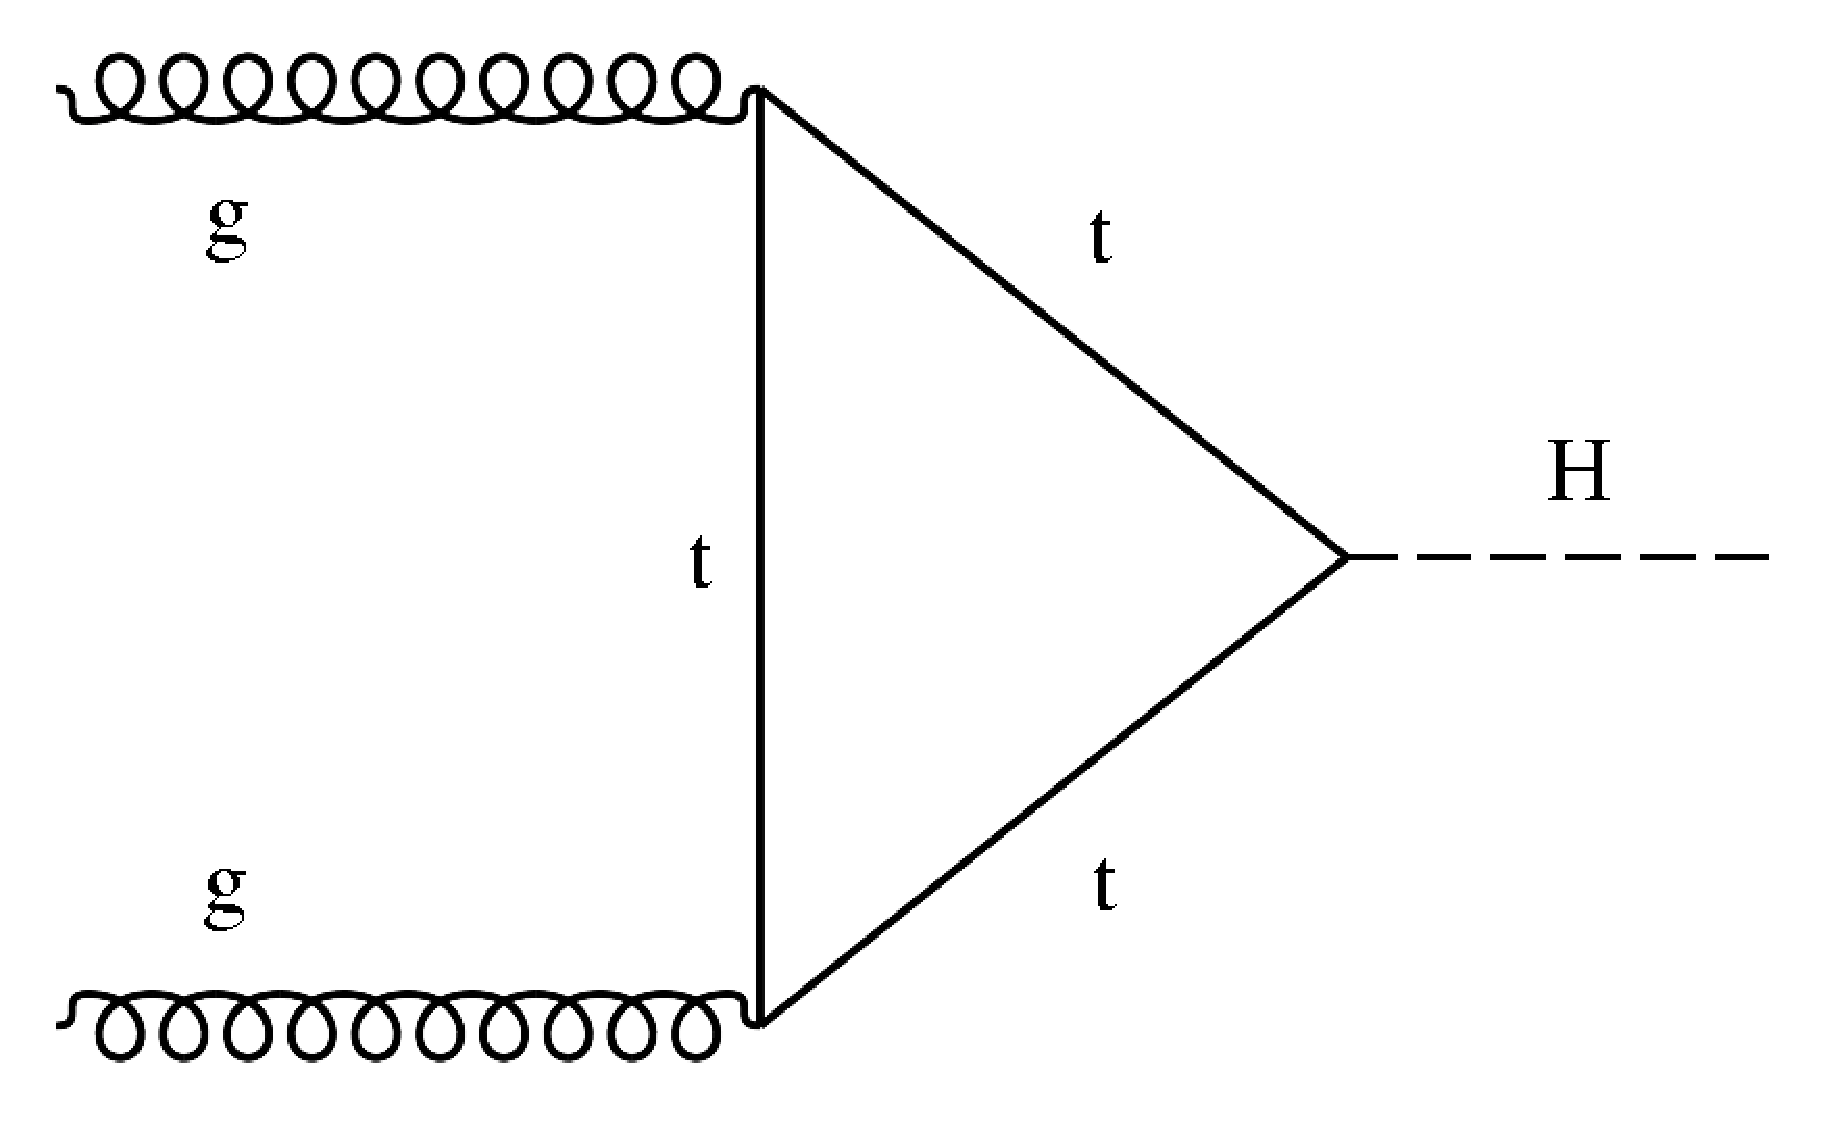
\includegraphics[width=0.47\linewidth]{figs/feynmanggH.pdf}

\end{figure}


%The Higgs boson decay to long-lived scalars is simulted using \PYTHIA v8.230~\cite{Sjostrand:2014zea}.
%The parton distribution functions used to produce all samples are the
%next-to-next-to-leading order (NNLO) NNPDF3.1 set~\cite{Ball:2017nwa}.
%For parton showering and hadronization, the matrix element generators are interfaced
%with \PYTHIA v8.230. For all samples, simulated additional pp interactions (pileup)
% are added to the hard-scattering process with the multiplicity distribution matched
% to the corresponding data-taking period (2016, 2017, 2018).
%The scalar is simulated as a generic scalar particle with a 100\% branching
%ratio to b-quarks (samples with scalar decays to light quarks and tau
%leptons also exist).
%We generate samples with varying scalar mass and lifetime, and include in this
%set of variations the
%benchmark points recommended by the LHCHXSWG~\cite{deFlorian:2016spz}.
Table~\ref{tab:sigsample} lists the signal Monte Carlo samples.

%%%%%%%%% %%%%%%%%%%%%%%%%%%%%%%%%%%%%%%%%%%%%%%%%%%%%%%%%%%%%%%%%%%%%%%%%%%%%%%%%
% The tables below are generated from lines like `python check_used.py | grep HToBB`
% using the script in LLDJstandalones/lists/ntuple
%%%%%%%%%%%%%%%%%%%%%%%%%%%%%%%%%%%%%%%%%%%%%%%%%%%%%%%%%%%%%%%%%%%%%%%%%%%%%%%%%%%%%%%%

\begin{table}[htb]
  %\caption{gg($h \rightarrow ss\rightarrow \tau\bar{\tau} \tau\bar{\tau}$) Signal Monte Carlo samples. Campaign is RunIIAutumn18MiniAOD-rp\_102X\_upgrade2018\_realistic\_v15-v1}
  \begin{center}
    %\footnotesize
    \scriptsize
    \begin{tabular}{l}\hline
      Sample \\
      \hline
      /ggH\_HToSSTo4Tau\_MH-125\_TuneCP5\_13TeV-powheg-pythia8/CAMPAIGN/MINIAODSIM\\
      \hline
      /ggH\_HToSSTo4Tau\_MH-125\_MS-55\_ctauS-1\_TuneCP5\_13TeV-powheg-pythia8/CAMPAIGN/MINIAODSIM\\
      /ggH\_HToSSTo4Tau\_MH-125\_MS-55\_ctauS-10\_TuneCP5\_13TeV-powheg-pythia8/CAMPAIGN/MINIAODSIM\\
      /ggH\_HToSSTo4Tau\_MH-125\_MS-55\_ctauS-100\_TuneCP5\_13TeV-powheg-pythia8/CAMPAIGN/MINIAODSIM\\
      /ggH\_HToSSTo4Tau\_MH-125\_MS-55\_ctauS-1000\_TuneCP5\_13TeV-powheg-pythia8/CAMPAIGN/MINIAODSIM\\
      /ggH\_HToSSTo4Tau\_MH-125\_MS-40\_ctauS-1\_TuneCP5\_13TeV-powheg-pythia8/CAMPAIGN/MINIAODSIM\\
      /ggH\_HToSSTo4Tau\_MH-125\_MS-40\_ctauS-10\_TuneCP5\_13TeV-powheg-pythia8/CAMPAIGN/MINIAODSIM\\
      /ggH\_HToSSTo4Tau\_MH-125\_MS-40\_ctauS-100\_TuneCP5\_13TeV-powheg-pythia8/CAMPAIGN/MINIAODSIM\\
      /ggH\_HToSSTo4Tau\_MH-125\_MS-40\_ctauS-1000\_TuneCP5\_13TeV-powheg-pythia8/CAMPAIGN/MINIAODSIM\\
      /ggH\_HToSSTo4Tau\_MH-125\_MS-15\_ctauS-1\_TuneCP5\_13TeV-powheg-pythia8/CAMPAIGN/MINIAODSIM\\
      /ggH\_HToSSTo4Tau\_MH-125\_MS-15\_ctauS-10\_TuneCP5\_13TeV-powheg-pythia8/CAMPAIGN/MINIAODSIM\\
      /ggH\_HToSSTo4Tau\_MH-125\_MS-15\_ctauS-100\_TuneCP5\_13TeV-powheg-pythia8/CAMPAIGN/MINIAODSIM\\
      /ggH\_HToSSTo4Tau\_MH-125\_MS-15\_ctauS-1000\_TuneCP5\_13TeV-powheg-pythia8/CAMPAIGN/MINIAODSIM\\
      /ggH\_HToSSTo4Tau\_MH-125\_MS-7\_ctauS-1\_TuneCP5\_13TeV-powheg-pythia8/CAMPAIGN/MINIAODSIM\\
      /ggH\_HToSSTo4Tau\_MH-125\_MS-7\_ctauS-10\_TuneCP5\_13TeV-powheg-pythia8/CAMPAIGN/MINIAODSIM\\
      /ggH\_HToSSTo4Tau\_MH-125\_MS-7\_ctauS-100\_TuneCP5\_13TeV-powheg-pythia8/CAMPAIGN/MINIAODSIM\\
      /ggH\_HToSSTo4Tau\_MH-125\_MS-7\_ctauS-1000\_TuneCP5\_13TeV-powheg-pythia8/CAMPAIGN/MINIAODSIM\\
      \hline
    \end{tabular}
    \label{tab:sigsample}
  \end{center}
\end{table}




%An example \PYTHIA v8.230 fragment for the Higgs decay to scalars (scalars) and their subsequent decay to tau leptons is given below.
%In this example the mass of the scalar is 15GeV and its lifetime (c$\tau$) is 10,000mm.
%\begin{verbatim}
%  '9000006:all = sk skbar 0 0 0 15 1.9732e-17 1.0 75.0 10000',
%  '9000006:oneChannel = 1  1.0 101  15 -15',
%  '9000006:mayDecay = on',
%  '9000006:isResonance = on',
%  '25:m0 = 125.0',
%  '25:onMode = off',
%  '25:addChannel = 1 0.000000001 101 9000006 -9000006',
%  '25:onIfMatch = 9000006 -9000006',
%  '9000006:onMode = off',
%  '9000006:onIfAny = 5',
%\end{verbatim}

\begin{figure}[h!]
  \caption{pt of the scalar products}
  \label{fig:scalarpt}
  \centering
  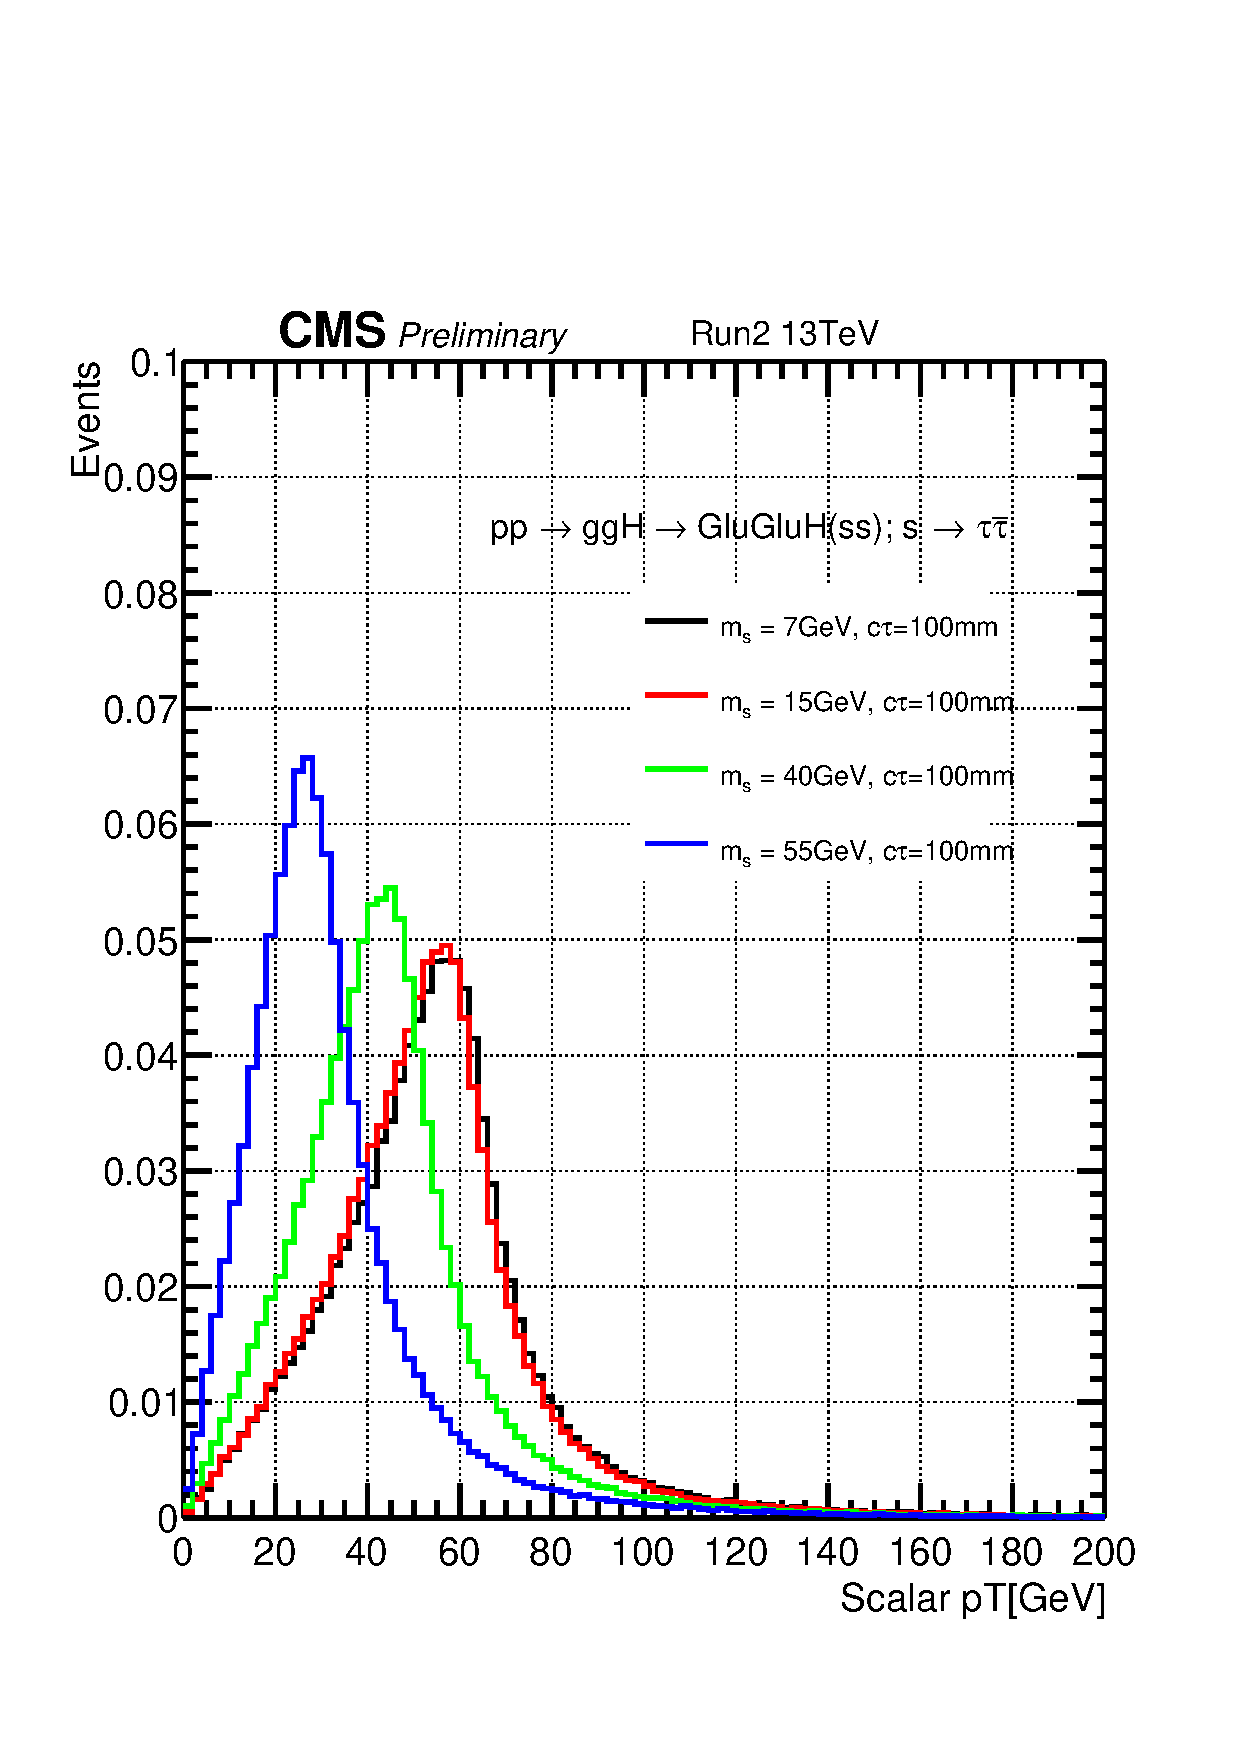
\includegraphics[width=0.47\linewidth]{figs/Scalar_pT100mm.pdf}
\end{figure}

\begin{figure}[h!]
  \caption{DeltaR of the scalar products}
  \label{fig:scalarpt}
  \centering
  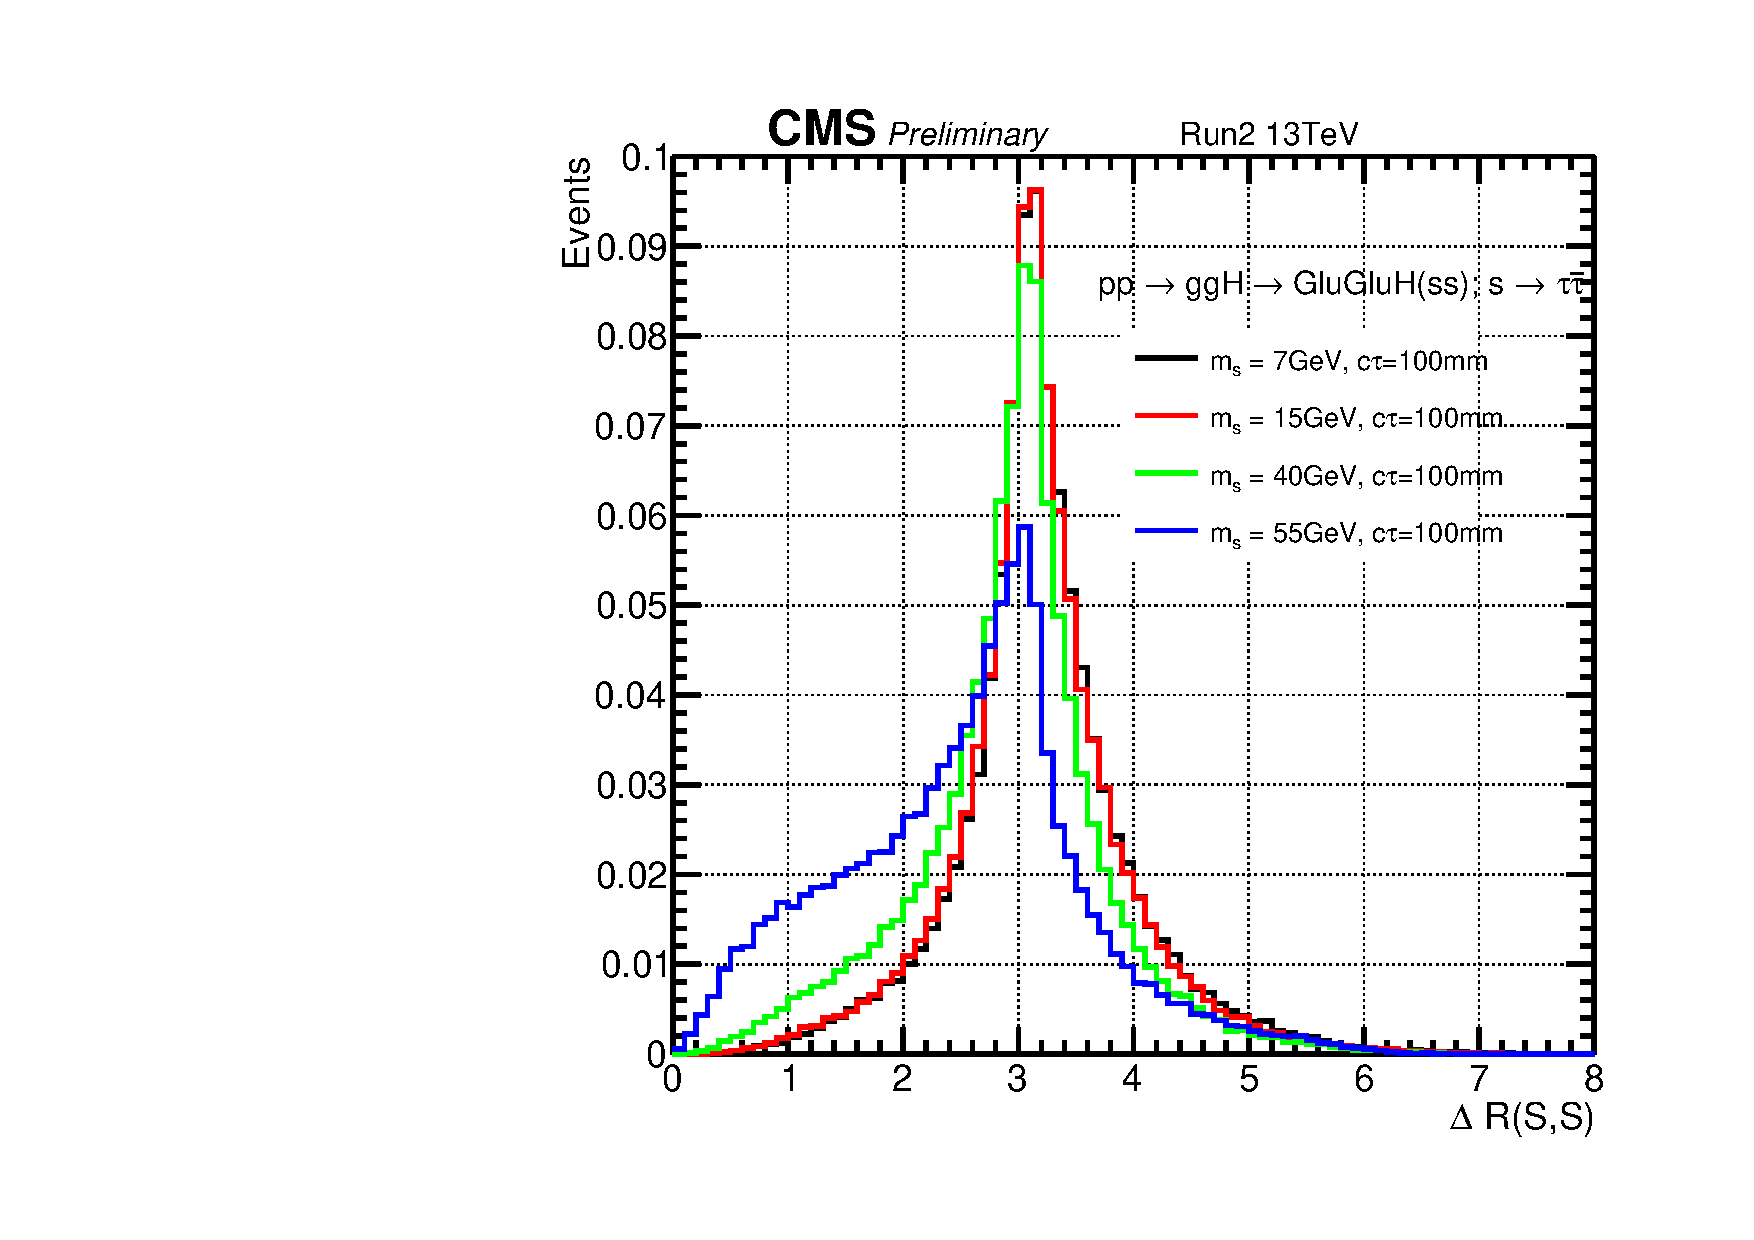
\includegraphics[width=0.47\linewidth]{figs/Scalar_dR100mm.pdf}
\end{figure}

\begin{figure}[h!]
  \caption{liftime of the scalar products in the lab frame}
  \label{fig:scalarpt}
  \centering
  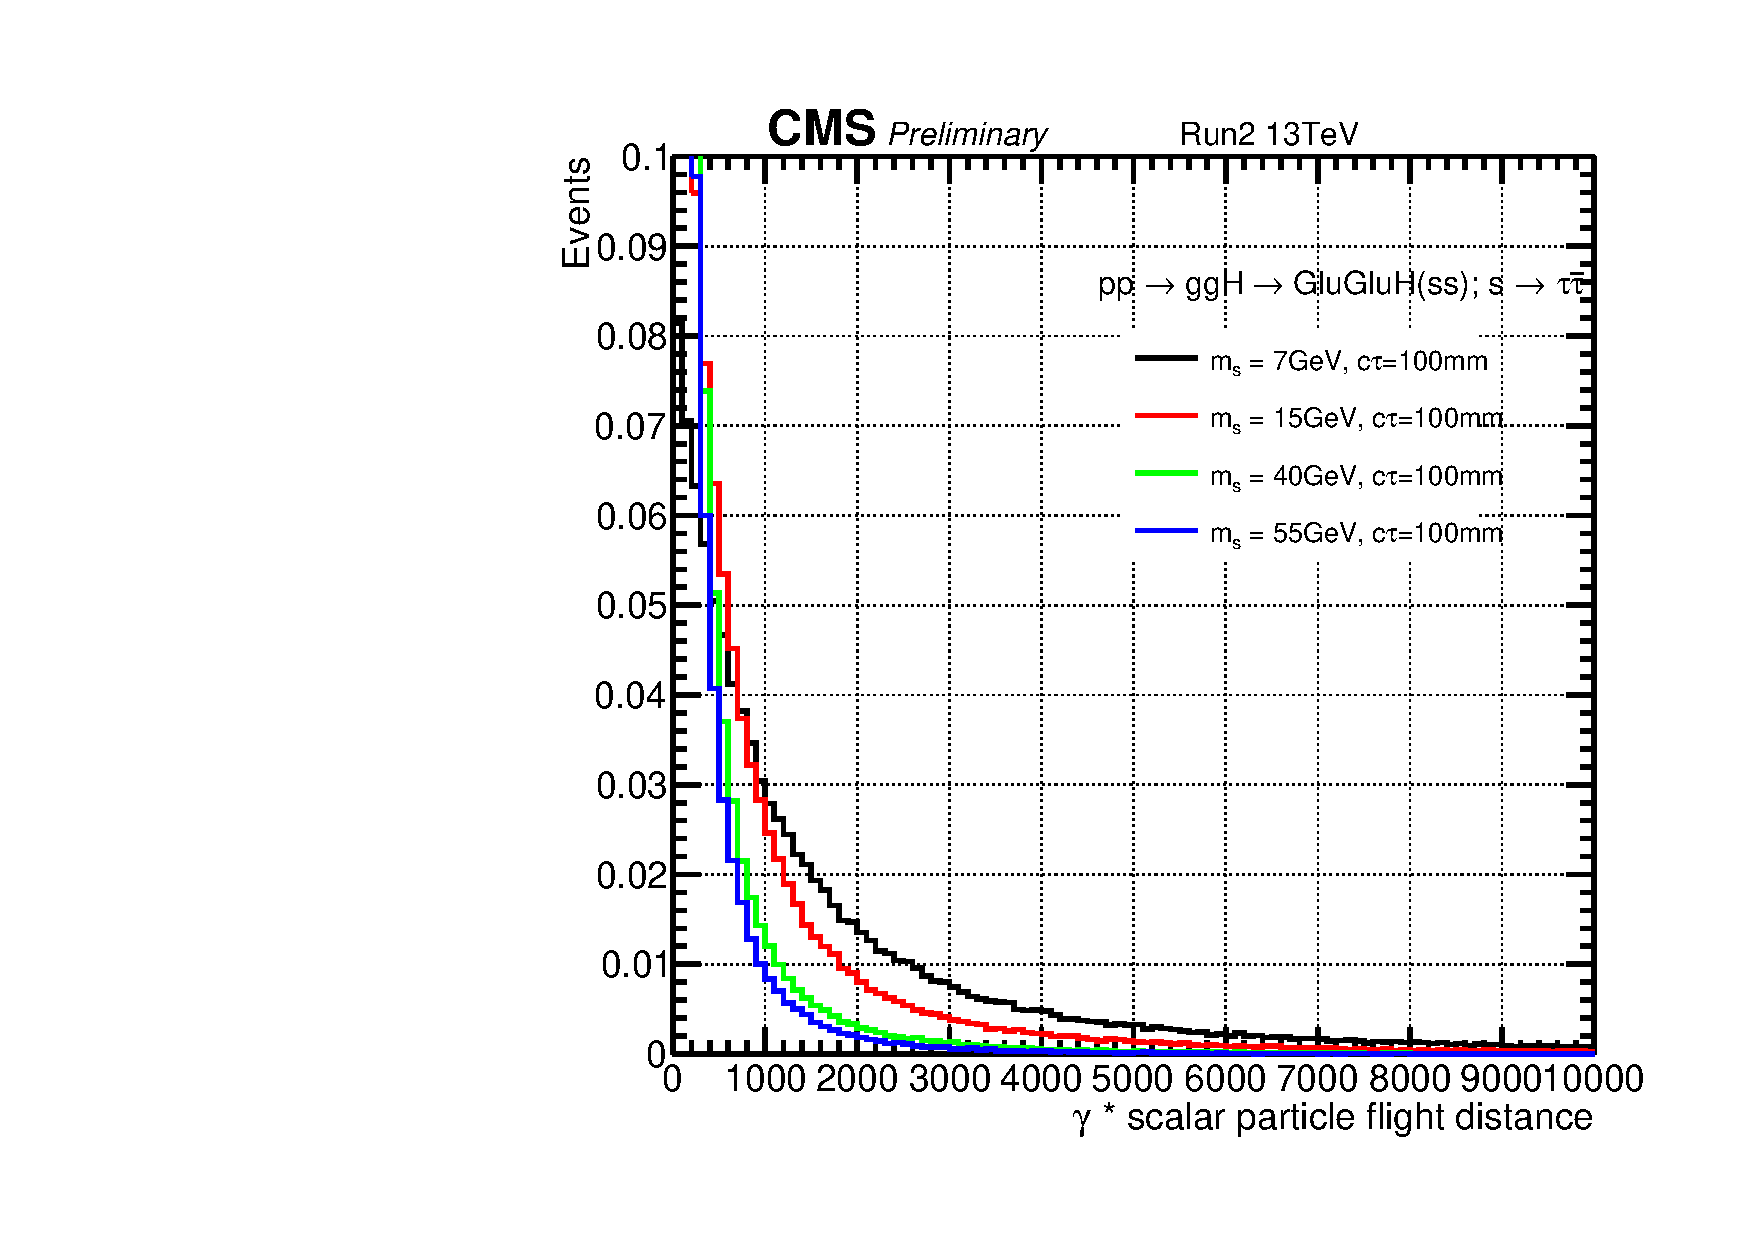
\includegraphics[width=0.47\linewidth]{figs/Scalar_gammactau100mm.pdf}
  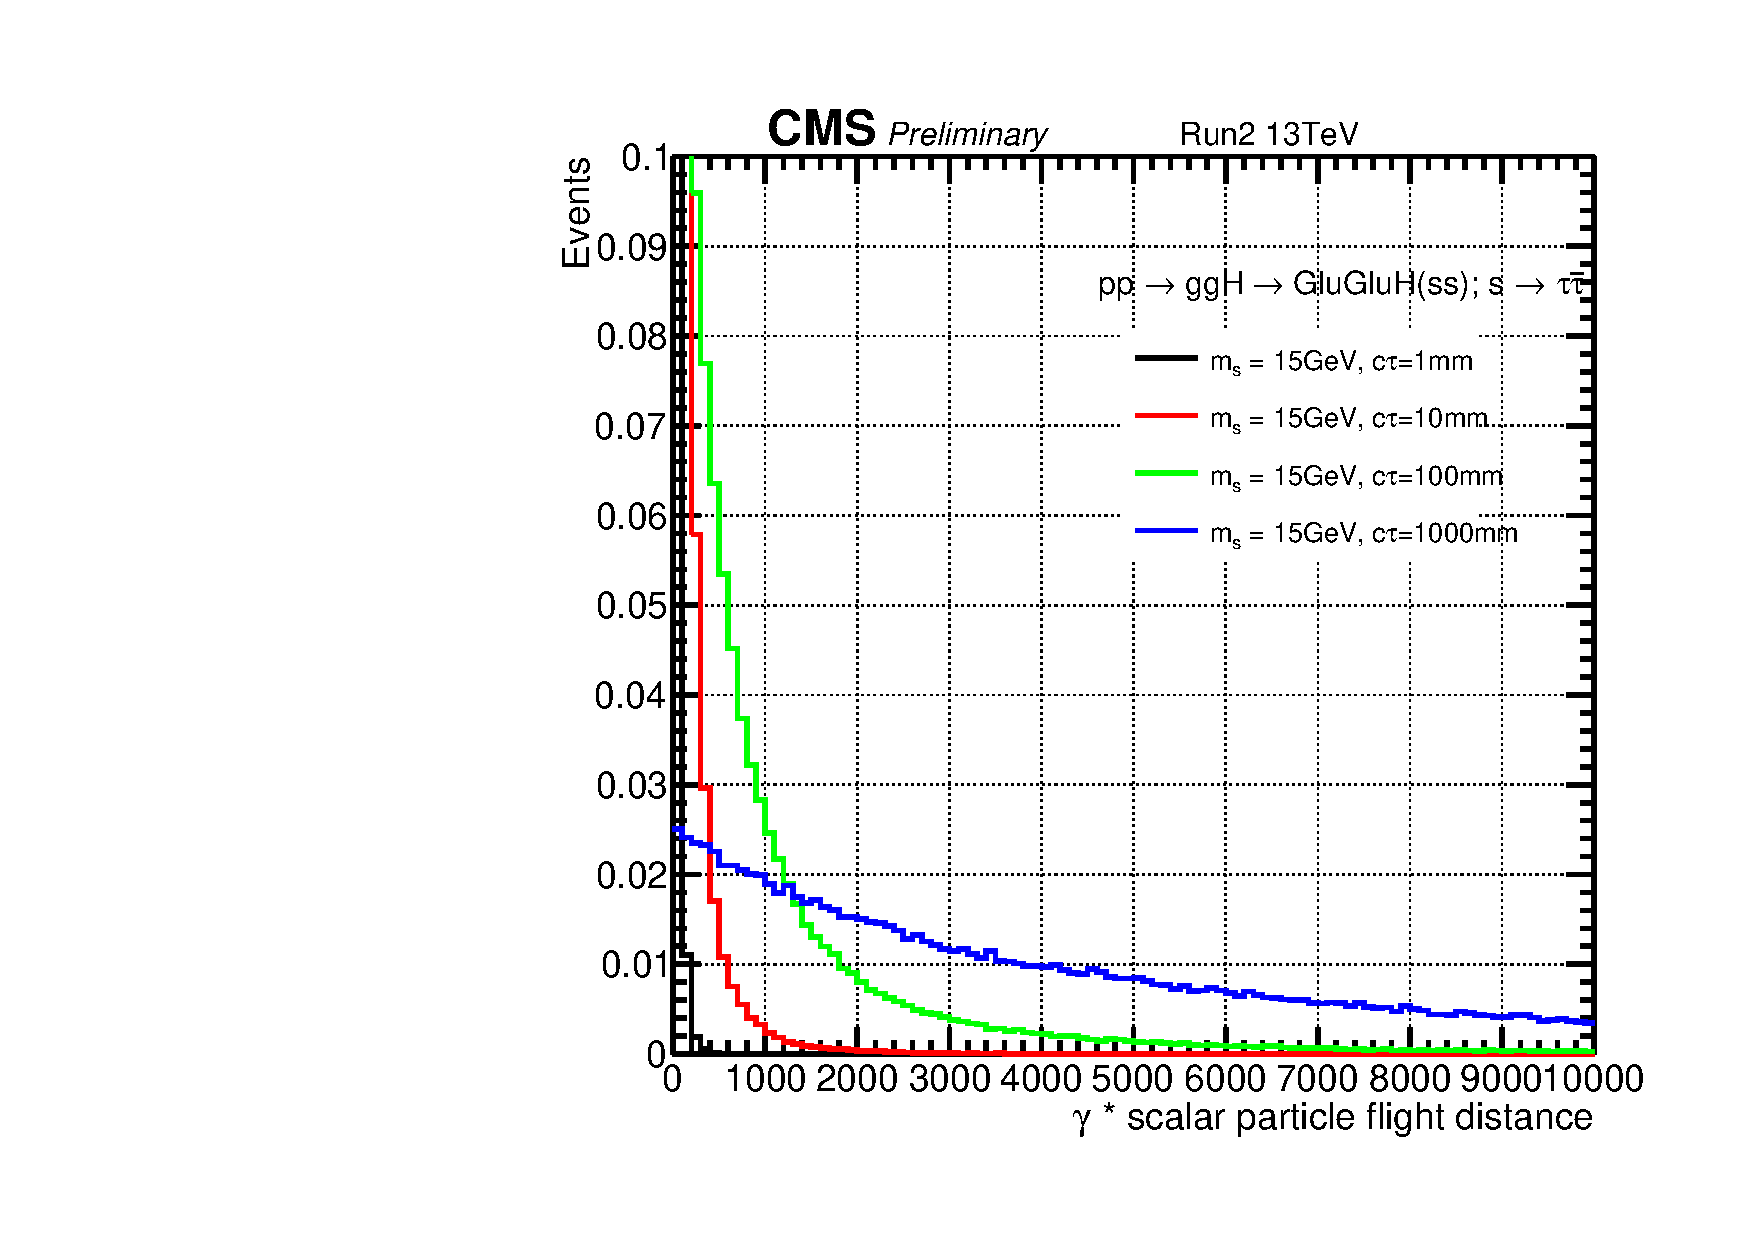
\includegraphics[width=0.47\linewidth]{figs/Scalar_gammactau15GeV.pdf}
\end{figure}






%Figure~\ref{fig:scalarpt} (left) and Figure~\ref{fig:zd_scalarpt} (left)
%show the Monte Carlo truth level distributions for the scalar ($S$) and $Z_{d}$ \pt, respectively.
%These distributions exhibit the soft-\pt nature of signal models.
%Figure~\ref{fig:scalarpt} (right) nd Figure~\ref{fig:zd_scalarpt} (right) show
% the Monte Carlo truth level distributions of the
%$\Delta R$ between the decay products of the scalar ($S$) and $Z_{d}$ for different masses.
%Note that significant portions of the distributions lie within the common jet radius of 0.4.
%Both of these figures show a signal with scalar decays to tau leptons to kinematically allow
%a lower scalar mass of 7GeV.
%
%\begin{figure}[h!]
%  \caption{\pt of the scalar ($s$) decay products (left) and
%  $\Delta R$ between the two scalar decay products (right) for different masses.
%  For the scalar masses below the $\mathrm{b}\mathrm{\bar{b}}$ threshold
%  the scalar decays into $\mathrm{d}\mathrm{\bar{d}}$.}
%  \label{fig:scalarpt}
%  \centering
%  %\includegraphics[width=0.47\linewidth]{figs/scalarpt.pdf}
%  %\includegraphics[width=0.45\linewidth]{figs/dr_lead_tautau.pdf}
%  \includegraphics[width=0.47\linewidth]{figs/dScalar_pT100mm.pdf}
%  \includegraphics[width=0.45\linewidth]{figs/dScalar_dR100mm.pdf}
%  %\SK placeholder\includegraphics[width=0.47\linewidth]{figs/Zdark_pT.pdf}
%  %\SK placeholder\includegraphics[width=0.45\linewidth]{figs/Zdark_dR.pdf}
%\end{figure}
%
%
%\begin{figure}[h!]
%  \caption{\pt of the $Z_{d}$ decay products (left)
%  and $\Delta R$ between the two $Z_{d}$ decay products (right) for different masses.}
%  \label{fig:zd_scalarpt}
%  \centering
%  \includegraphics[width=0.47\linewidth]{figs/Zdark_pT.pdf}
%  \includegraphics[width=0.47\linewidth]{figs/Zdark_dR.pdf}
%\end{figure}
%
%
%Figure~\ref{fig:flightdist} and Figure~\ref{fig:zd_flightdist} show the flight distances in the lab-frame
%for different scalar ($S$) and $Z_{d}$ proper-lifetimes, respectively.
%Figure~\ref{fig:Zdark_pT} shows the Z boson \pt distribution for different
%heavy scalar ($\Phi$) and $Z_{d}$ masses. The Z boson \pt starts to be well above
%the 100GeV threshold set by the background estimation method (see Section~\ref{sec:searhregion})
%for $\Phi$ masses ($m_{\Phi}$) above 250GeV. Therefore, we focus the model interpretation
%in the scenarios where $m_{\Phi} > 250$GeV.
%
%\begin{figure}[h!]
%  \caption{LLP flight distance in lab-frame for different scalar lifetimes and masses.
%  For the scalar masses below the $\mathrm{b}\mathrm{\bar{b}}$ threshold
%  the scalar decays into $\mathrm{d}\mathrm{\bar{d}}$.
%  }
%  \label{fig:flightdist}
%  \centering
%  \includegraphics[width=0.47\linewidth]{figs/dScalar_dist_7GeV.pdf}
%  \includegraphics[width=0.47\linewidth]{figs/Scalar_MS15.pdf}
%  \includegraphics[width=0.47\linewidth]{figs/Scalar_MS40.pdf}
%  \includegraphics[width=0.47\linewidth]{figs/Scalar_MS55.pdf}
%\end{figure}
%
%\begin{figure}[h!]
%  \caption{LLP flight distance in lab-frame for different $Z_{d}$ lifetimes and masses.
%   Information is MC-thruth
%  }
%  \label{fig:zd_flightdist}
%  \centering
%  \includegraphics[width=0.47\linewidth]{figs/Zd_ctau_llp20.pdf}
%  \includegraphics[width=0.47\linewidth]{figs/Zd_ctau_llp50.pdf}
%\end{figure}
%
%\begin{figure}[h!]
%  \caption{$Z$ $p_{T}$ comparison for a scalar mass ($\Phi$) of 50GeV.
%   $Z_{d}$ mass of  20GeV (left)  and 50GeV (right).
%  }
%  \label{fig:Zdark_pT}
%  \centering
%  \includegraphics[width=0.47\linewidth]{figs/Zdark_Zpt175llp20.pdf}
%  \includegraphics[width=0.47\linewidth]{figs/Zdark_Zpt175llp50.pdf}
%\end{figure}

\subsection{Background Monte Carlo}
All samples were processed as recommended in the PPD Run2 Analysis Guideline~\cite{pdmv}.
Tables~\ref{tab:QCDsample}-\ref{tab:18samplesummary} summarizes the background Monte Carlo used in this analysis.

%%%%%%%%%%%%%%%%%%%%%%%%%%
%%%%%%%%%2018%%%%%%%%%%%%%
%%%%%%%%%%%%%%%%%%%%%%%%%%
\begin{table}[htb]
  \caption{QCD MuEnriched Pt5 background Monte Carlo samples}
  \begin{center}
    \footnotesize
    %\scriptsize
    \begin{tabular}{l}\hline
      Sample \\
      \hline
      /QCD\_Pt-15to20\_MuEnrichedPt5\_TuneCP5\_13TeV\_pythia8/*-v3/MINIAODSIM \\
      /QCD\_Pt-20to30\_MuEnrichedPt5\_TuneCP5\_13TeV\_pythia8/*-v4/MINIAODSIM \\
      /QCD\_Pt-30to50\_MuEnrichedPt5\_TuneCP5\_13TeV\_pythia8/*-v3/MINIAODSIM \\
      /QCD\_Pt-50to80\_MuEnrichedPt5\_TuneCP5\_13TeV\_pythia8/*-v3/MINIAODSIM \\
      /QCD\_Pt-80to120\_MuEnrichedPt5\_TuneCP5\_13TeV\_pythia8/*\_ext1-v2/MINIAODSIM \\
      /QCD\_Pt-120to170\_MuEnrichedPt5\_TuneCP5\_13TeV\_pythia8/*\_ext1-v2/MINIAODSIM \\
      /QCD\_Pt-170to300\_MuEnrichedPt5\_TuneCP5\_13TeV\_pythia8/*-v3/MINIAODSIM \\
      /QCD\_Pt-300to470\_MuEnrichedPt5\_TuneCP5\_13TeV\_pythia8/*\_ext3-v1/MINIAODSIM \\
      /QCD\_Pt-470to600\_MuEnrichedPt5\_TuneCP5\_13TeV\_pythia8/*\_ext1-v2/MINIAODSIM \\
      /QCD\_Pt-600to800\_MuEnrichedPt5\_TuneCP5\_13TeV\_pythia8/*-v1/MINIAODSIM \\
      /QCD\_Pt-800to1000\_MuEnrichedPt5\_TuneCP5\_13TeV\_pythia8/*\_ext3-v2/MINIAODSIM \\
      /QCD\_Pt-1000toInf\_MuEnrichedPt5\_TuneCP5\_13TeV\_pythia8/*-v1/MINIAODSIM \\
      \hline
    \end{tabular}
    \label{tab:QCDsample}
  \end{center}
\end{table}
a


\begin{table}[htb]
  \caption{W,Z,H boson background Monte Carlo samples}
  \begin{center}
    \footnotesize
    \begin{tabular}{l}\hline
      Sample \\
      \hline
      /DYJetsToLL\_M-50\_TuneCP5\_13TeV-madgraphMLM-pythia8/*-v1/MINIAODSIM \\
      \hline
      /WJetsToLNu\_M-50\_TuneCP5\_13TeV-madgraphMLM-pythia8/*-v2/MINIAODSIM \\
      \hline
      /WW\_M-50\_TuneCP5\_13TeV-madgraphMLM-pythia8/*-v2/MINIAODSIM \\
      /WZ\_M-50\_TuneCP5\_13TeV-madgraphMLM-pythia8/*-v3/MINIAODSIM \\
      /ZZ\_M-50\_TuneCP5\_13TeV-madgraphMLM-pythia8/*-v2/MINIAODSIM \\
      \hline
      /GluGluHToBB\_M125\_13TeV\_amcatnloFXFX\_pythia8/*-v1/MINIAODSIM \\
      \hline
    \end{tabular}
    \label{tab:wzsample}
  \end{center}
\end{table}


\begin{table}[htb]
  \caption{Top background Monte Carlo samples}
  \begin{center}
    \footnotesize
    \begin{tabular}{l}\hline
      Sample \\
      \hline
      /TTJets\_TuneCP5\_13TeV-madgraphMLM-pythia8/*-v1/MINIAODSIM \\
      \hline
      /ST\_s-channel\_4f\_hadronicDecays\_TuneCP5\_13TeV-madgraph-pythia8/*\_ext1-v1/MINIAODSIM \\
      /ST\_t-channel\_top\_5f\_TuneCP5\_13TeV-powheg-pythia8/*-v1/MINIAODSIM \\
      /ST\_t-channel\_antitop\_5f\_TuneCP5\_13TeV-powheg-pythia8/*-v1/MINIAODSIM \\
      /ST\_tW\_antitop\_5f\_inclusiveDecays\_TuneCP5\_13TeV-powheg-pythia8/*\_ext1-v1/MINIAODSIM \\
      /ST\_tW\_top\_5f\_inclusiveDecays\_TuneCP5\_13TeV-powheg-pythia8/*\_ext1-v1/MINIAODSIM \\
      \hline
    \end{tabular}
    \label{tab:topsample}
  \end{center}
\end{table}


\begin{table}[htb]
  \caption{Monte Carlo sample summary}
  \begin{center}
    \footnotesize
    %\scriptsize
    \begin{tabular}{l}\hline
      Sample \\
      \hline
      /QCD\_Pt-15to20\_MuEnrichedPt5\_TuneCP5\_13TeV\_pythia8/*-v3/MINIAODSIM \\
      /QCD\_Pt-20to30\_MuEnrichedPt5\_TuneCP5\_13TeV\_pythia8/*-v4/MINIAODSIM \\
      /QCD\_Pt-30to50\_MuEnrichedPt5\_TuneCP5\_13TeV\_pythia8/*-v3/MINIAODSIM \\
      /QCD\_Pt-50to80\_MuEnrichedPt5\_TuneCP5\_13TeV\_pythia8/*-v3/MINIAODSIM \\
      /QCD\_Pt-80to120\_MuEnrichedPt5\_TuneCP5\_13TeV\_pythia8/*\_ext1-v2/MINIAODSIM \\
      /QCD\_Pt-120to170\_MuEnrichedPt5\_TuneCP5\_13TeV\_pythia8/*\_ext1-v2/MINIAODSIM \\
      /QCD\_Pt-170to300\_MuEnrichedPt5\_TuneCP5\_13TeV\_pythia8/*-v3/MINIAODSIM \\
      /QCD\_Pt-300to470\_MuEnrichedPt5\_TuneCP5\_13TeV\_pythia8/*\_ext3-v1/MINIAODSIM \\
      /QCD\_Pt-470to600\_MuEnrichedPt5\_TuneCP5\_13TeV\_pythia8/*\_ext1-v2/MINIAODSIM \\
      /QCD\_Pt-600to800\_MuEnrichedPt5\_TuneCP5\_13TeV\_pythia8/*-v1/MINIAODSIM \\
      /QCD\_Pt-800to1000\_MuEnrichedPt5\_TuneCP5\_13TeV\_pythia8/*\_ext3-v2/MINIAODSIM \\
      /QCD\_Pt-1000toInf\_MuEnrichedPt5\_TuneCP5\_13TeV\_pythia8/*-v1/MINIAODSIM \\
      /DYJetsToLL\_M-50\_TuneCP5\_13TeV-madgraphMLM-pythia8/*-v1/MINIAODSIM \\
      /WJetsToLNu\_M-50\_TuneCP5\_13TeV-madgraphMLM-pythia8/*-v2/MINIAODSIM \\
      /WW\_M-50\_TuneCP5\_13TeV-madgraphMLM-pythia8/*-v2/MINIAODSIM \\
      /WZ\_M-50\_TuneCP5\_13TeV-madgraphMLM-pythia8/*-v3/MINIAODSIM \\
      /ZZ\_M-50\_TuneCP5\_13TeV-madgraphMLM-pythia8/*-v2/MINIAODSIM \\
      /GluGluHToBB\_M125\_13TeV\_amcatnloFXFX\_pythia8/*-v1/MINIAODSIM \\
      /TTJets\_TuneCP5\_13TeV-madgraphMLM-pythia8/*-v1/MINIAODSIM \\
      /ST\_s-channel\_4f\_hadronicDecays\_TuneCP5\_13TeV-madgraph-pythia8/*\_ext1-v1/MINIAODSIM \\
      /ST\_t-channel\_top\_5f\_TuneCP5\_13TeV-powheg-pythia8/*-v1/MINIAODSIM \\
      /ST\_t-channel\_antitop\_5f\_TuneCP5\_13TeV-powheg-pythia8/*-v1/MINIAODSIM \\
      /ST\_tW\_antitop\_5f\_inclusiveDecays\_TuneCP5\_13TeV-powheg-pythia8/*\_ext1-v1/MINIAODSIM \\
      /ST\_tW\_top\_5f\_inclusiveDecays\_TuneCP5\_13TeV-powheg-pythia8/*\_ext1-v1/MINIAODSIM \\
      \hline
      /ggH\_HToSSTo4Tau\_MH-125\_TuneCP5\_13TeV-powheg-pythia8/*-v1/MINIAODSIM\\
      \hline
    \end{tabular}
    \label{tab:18samplesummary}
  \end{center}
\end{table}












\chapter{Others}

